%%%%%%%%%%%%%%%%%%%%%%%%%%%%%%%%%%%%%%%%%
% Beamer Presentation
% LaTeX Template
% Version 1.0 (10/11/12)
%
% This template has been downloaded from:
% http://www.LaTeXTemplates.com
%
% License:
% CC BY-NC-SA 3.0 (http://creativecommons.org/licenses/by-nc-sa/3.0/)
%
%%%%%%%%%%%%%%%%%%%%%%%%%%%%%%%%%%%%%%%%%
\documentclass{beamer}

\mode<presentation> {
\usetheme{Madrid}
\usefonttheme{serif} 
\setbeamertemplate{navigation symbols}{} 
}
\usepackage{graphicx} % Allows including images
\usepackage{booktabs} % Allows the use of \toprule, \midrule and \bottomrule in tables
\usepackage[T1]{fontenc}
\usepackage[utf8]{inputenc}
\usepackage{amsmath}
\usepackage{color}
\usepackage[czech]{babel}
\usepackage{lmodern}  
\usepackage{rotating}
\usepackage{scrextend}
\usepackage{pifont}
\usepackage{hyperref}
\usepackage{bm}

%----------------------------------------------------------------------------------------
%	TITLE PAGE
%----------------------------------------------------------------------------------------

\title[Týden 5]{Praktikum z ekonometrie} % The short title appears at the bottom of every slide, the full title is only on the title page

\author{VŠE Praha} % Your name
\institute[4EK417] % Your institution as it will appear on the bottom of every slide, may be shorthand to save space
{
% Your institution for the title page
\medskip
\textit{Tomáš Formánek} % Your email address
}
\date{} % Date, can be changed to a custom date

\begin{document}

\begin{frame}
\titlepage % Print the title page as the first slide
\end{frame}

\begin{frame}
\frametitle{Outline} % Table of contents slide, comment this block out to remove it
\tableofcontents % Throughout your presentation, if you choose to use \section{} and \subsection{} commands, these will automatically be printed on this slide as an overview of your presentation
\end{frame}
%	PRESENTATION SLIDES
%---------------------------------------------------------------------
\section{Introduction}
\begin{frame}{Introduction}
\end{frame}
%---------------------------------------------------------------------
\begin{frame}{Introduction - spatial analysis}
\begin{figure}
	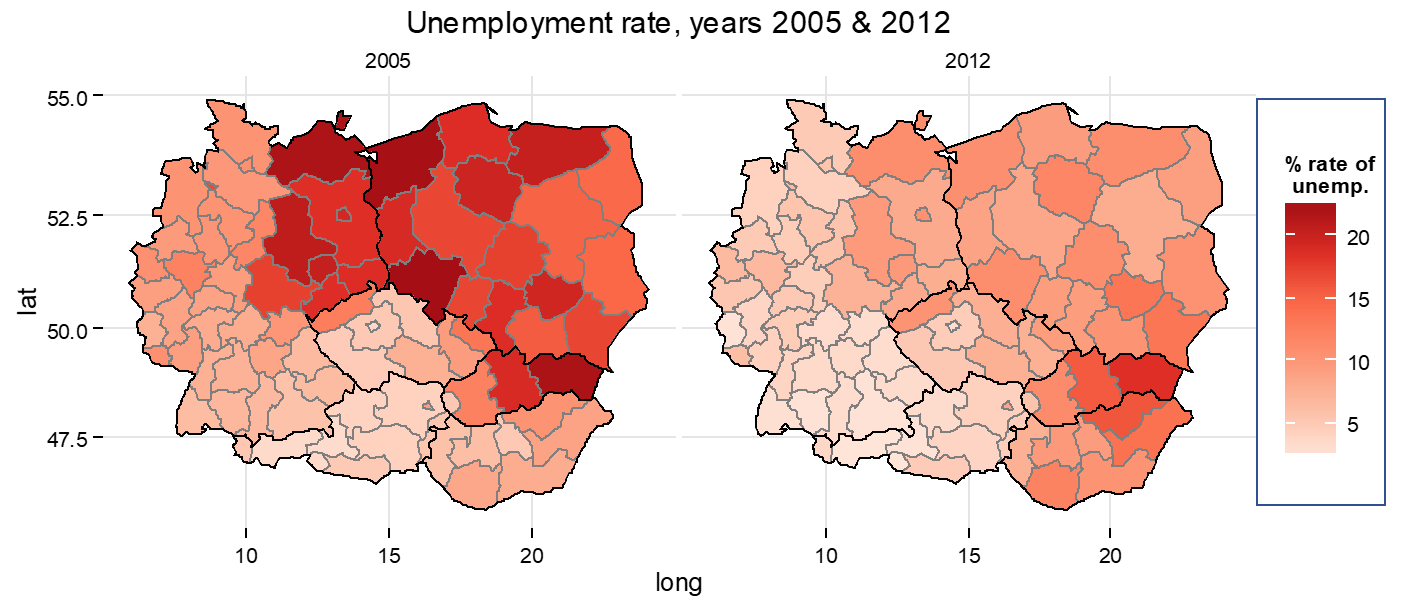
\includegraphics[width=.9\textwidth]{IMG/sp_auto2.PNG}
\end{figure}
\end{frame}
%---------------------------------------------------------------------
\begin{frame}{Introduction - spatial analysis}
Methods of quantitative spatial analysis:\\
\bigskip
\begin{itemize}
    \item Visualization \\Maps, graphical display
    \bigskip
    \item Data exploration \& descriptive methods \\Tools to broadly look at spatial patterns
    \bigskip
    \item Econometric modeling \\Fitting models, testing hypotheses, formalizing spatial dependence, discerning spatial effects from other factor (e.g. macroeconomic)
\end{itemize}
\end{frame}
%---------------------------------------------------------------------
\begin{frame}{Introduction - spatial analysis}
 What are spatial data?\\
\bigskip
\begin{itemize}
    \item Data that are location speciffic and that vary in space.
    \medskip
    \item Referenced by a spatial location $\bm{s}$ (usually 2D),  \\$\bm{s} = (x; y)$; $x$ is longitude (easting) and $y$ is latitude (northing). \\ \medskip
    May also be referenced by a zip code, county or state ID.
    \medskip
    \item Data that are close together in space (time) are often more alike than those that are far apart.
    \medskip
    \item Tobler's first law of geography: \\ ``Everything is related to everything else, but near things are more related than distant things.''
\end{itemize}
\end{frame}
%---------------------------------------------------------------------
\begin{frame}{History of spatial analysis: 1854 -- London -- cholera}
\vspace{-0.5cm}
\begin{figure}
	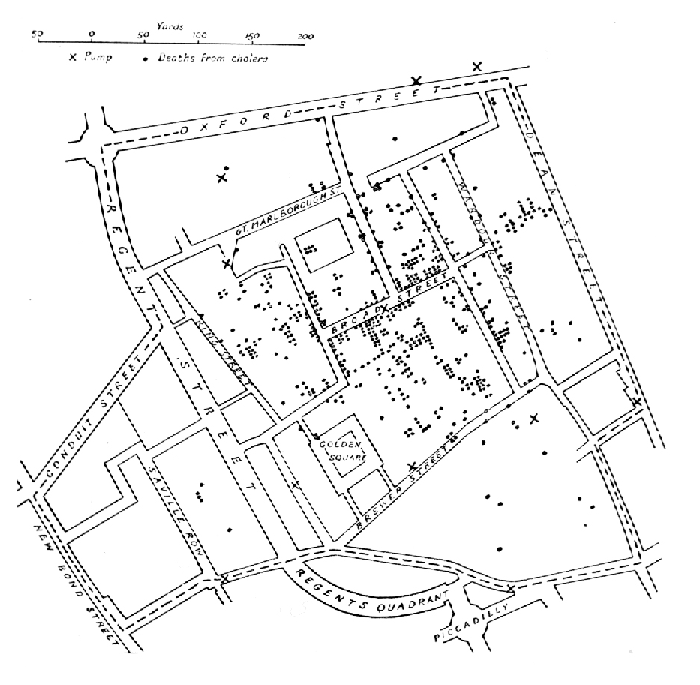
\includegraphics[width=.65\textwidth]{IMG/sp_cholera.eps}
\end{figure}
\end{frame}
%---------------------------------------------------------------------
\begin{frame}{History of spatial analysis: 1854 -- London -- cholera}
 Dr. John Snow: Early spatial analysis\\
\medskip
\begin{itemize}
    \item In August 1854, there was a major Cholera outbreak in the Soho neighbourhood of London, UK. There were 127 cholera related deaths around the area.
    \smallskip
    \item At the time, germ theory (microorganisms causing disease) was not generally accepted. Dr. J. Snow was a MD, pioneer of germ theory and a statistician.
    \smallskip
    \item Dr. John Snow spoke to local residents and mapped where cholera cases occurred. As a result of his map, he was able to pinpoint the public water pump on Broad Street as the source of contaminated water causing the cholera outbreak.
    \smallskip
    \item Dr. Snow used statistics to find a relationship between water sources and cholera cases and subsequently found out that the waterworks company supplying water to Broad Street pump was taking water from a sewage polluted area of the Thames river.
\end{itemize}
\end{frame}
%---------------------------------------------------------------------
\begin{frame}{History of spatial analysis: 1935 -- field experiments}
\vspace{-0.5cm}
\begin{figure}
	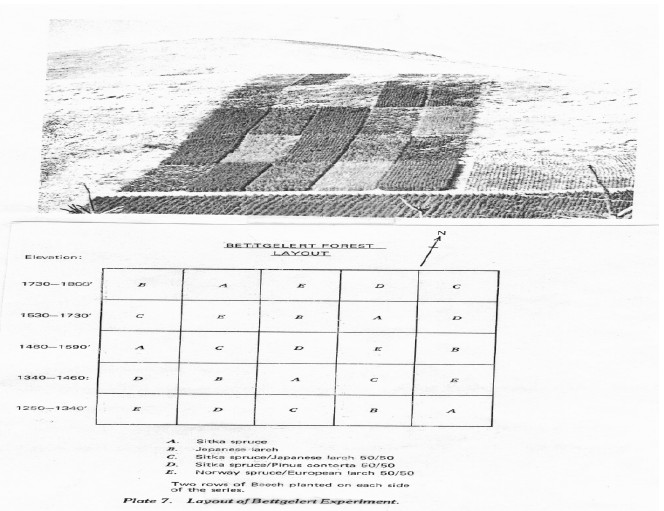
\includegraphics[width=.8\textwidth]{IMG/sp_Fisher.jpg}
\end{figure}
\end{frame}
%---------------------------------------------------------------------
\begin{frame}{History of spatial analysis: 1935 -- field experiments}
 R.A. Fisher: Early spatial analysis\\
\medskip
\begin{itemize}
    \item R.A. Fisher was probably the first to recognize implications of spatial dependency for statistical analysis.
    \smallskip
    \item In his work on design of experiments in agricultural science, he wrote (Fisher, 1935, p. 66):\\
    ``After choosing the area we usually have no guidance beyond the widely verified fact that patches in close proximity are commonly more alike, as judged by the yield of crops, than those which are further apart.''
    \smallskip
    \item Observed spatial variability, i.e. field-to-field variability, was largely due to physical properties of the soil and environmental properties of the field. He avoided the confounding of treatment effects with plot effect with the introduction of randomization.
    \smallskip
    \item Fisher's solution was to eliminate spatial dependency bias by localizing the crops under scrutiny into randomly assigned blocks.
\end{itemize}
\end{frame}
%---------------------------------------------------------------------
\section{Spatial stochastic processes}
\begin{frame}{Spatial stochastic processes}
\end{frame}
%---------------------------------------------------------------------
\begin{frame}{Measuring spatial variables}
Spatial data: measurements and measurement scales
\begin{itemize}
    \item \textbf{Generally, data vary continuously over space, but are measured only at discrete locations.} 
    \begin{itemize}
        \item To characterize spatial variables, spatial aggregation is necessary.
        \item Aggregation of spatial variables may be just another source of bias and potential data mis-manipulation\\ 
        Summary values are influenced by shape and scale of spatial units.\\
        Shape (administrative boundaries) may change over time.
    \end{itemize}
    \item Scale, consistency and relevance should be carefully considered
when collecting and analyzing spatial data
\end{itemize}
\medskip
Spatio-temporal data:
\begin{itemize}
    \item Data that are location specific and repeated in time.
    \item Each variable-observation has a location, time and value.
    \item Similar methods for analysis, with an added time dimension \\(choice of sampling frequency, spatial panel data analysis)
\end{itemize}
\end{frame}
%---------------------------------------------------------------------
\begin{frame}{Measuring spatial distances}
Distances ($d$) can be defined in a variety of ways, yet the following technical conditions should always apply (invariant to spatial translation, i.e. ``shift''):\\
\medskip
\begin{enumerate} 
\item[1] $d(\bm{s}_i, \bm{s}_j) = d(\bm{s}_j, \bm{s}_i)$ \\ \smallskip (symmetry) 
\medskip
\item[2] $d(\bm{s}_i, \bm{s}_i) = 0$  \\ \smallskip (dist. between a point and itself is zero) 
\medskip
\item[3] $d(\bm{s}_i, \bm{s}_j) \leq d(\bm{s}_i) + d(\bm{s}_j)$  \\ \smallskip (triangle inequality; 
$d(\bm{s}_i)$ is the distance from origin) 
\end{enumerate}
\end{frame}
%---------------------------------------------------------------------
\begin{frame}{Measuring spatial distances}
Distances ($d$) can be defined in a variety of ways, yet the following technical conditions should always apply (invariant to spatial translation, i.e. ``shift''):\\
\medskip
\begin{enumerate} 
\item[1] $d(\bm{s}_i, \bm{s}_j) = d(\bm{s}_j, \bm{s}_i)$ \\ \smallskip (symmetry) 
\medskip
\item[2] $d(\bm{s}_i, \bm{s}_i) = 0$  \\ \smallskip (dist. between a point and itself is zero) 
\medskip
\item[3] $d(\bm{s}_i, \bm{s}_j) \leq d(\bm{s}_i) + d(\bm{s}_j)$  \\ \smallskip (triangle inequality; 
$d(\bm{s}_i)$ is the distance from origin) 
\end{enumerate}
\end{frame}
%---------------------------------------------------------------------
\begin{frame}{Measuring spatial distances}
\small{\textbf{Euclidean distances}, measured between two point in the ``ordinary'' Euclidean space. In 2D, the Euclidean distance ($L_2$ norm) is defined as 
$$
d(\bm{s}_i, \bm{s}_j) = \sqrt[]{(s_{ix}-s_{jx})^2+(s_{iy}-s_{jy})^2}\,,
$$
where the $x$ and $y$ subscripts handle planar coordinates. For smaller distances, the computational simplicity is attractive.\\
\medskip
\textbf{Great circle distances} - for larger distances, planar projection accumulates non-negligible errors. The shortest path between two points on a sphere (given their longitudes and latitudes): 
$$
d(\bm{s}_i, \bm{s}_j) = 2r \, \arcsin \,
 \sqrt{ \sin^2 \left( \frac{\phi_j-\phi_i}{2} \right)
       + \cos(\phi_i) \cos(\phi_j)
       \sin^2 \left( \frac{l_j-l_i}{2} \right) }\,,
$$
where $r$ is the radius of the sphere, $\phi_1$ and $\phi_2$ are the latitudes of $\bm{s}_i$ and $\bm{s}_j$ in radians, $l_i$ and $l_j$ are the longitudes (in radians). Its only an approximation when applied to the Earth, which is not a perfect sphere (correct within a 0.5\%; alternative: Vicenty's formulae).\\
\medskip
\textbf{Manhatan distances} - $L_1$ norm, a function on a fixed grid.
}
\end{frame}
%---------------------------------------------------------------------
\begin{frame}{Spatial stochastic processes}
For a generic location $\bm{s}$ given by a vector of $d$ coordinates in a $d$-dimensional Euclidean space, spatial stochastic process \\(``random field'') is often denoted as
$$ Z(\bm{s}): \bm{s} \in D \subseteq \mathbb{R}^d \, .$$
\vspace{-0.5cm}
\begin{itemize}
    \item Typically, $d=2$ for most economic and econometric applications, $d=3$ is often used in fields such as geology or astronomy. 
    \smallskip
    \item $D$ is a fixed finite set of $N$ spatial locations $\bm{s}_1, \bm{s}_2, \dots, \bm{s}_N$. 
    \smallskip
    \item Individual $\bm{s}_i$ units are points in space (say, with GPS-based latitude and longitude coordinates). Sometimes, such points can be associated with non-zero surface area elements.
    \item Much like in time-series analysis, the individual realizations of a spatial stochastic process -- random field -- are often denoted \\$z(\bm{s}_i)$ or, simply, $z_i$.
\end{itemize}
\end{frame}
%---------------------------------------------------------------------
\begin{frame}{Spatial stochastic processes}
Stationarity is a common assumption: a spatial process under scrutiny repeats itself over the domain $D$. If we translate the entire set of coordinates by $\bm{h}$ -- a specific distance in a specified direction, the stochastic process and its features remain unchanged.\\
\medskip
\textbf{Strong stationarity} of a random filed: We start with a finite-dimensional distribution: 
$$F_{\bm{s}_1, \dots,\bm{s}_m }(z_1,\dots, z_m) = P[Z(\bm{s}_1) \leq z_1, Z(\bm{s}_2) \leq z_2, \dots, Z(\bm{s}_m) \leq z_m] \, .$$  
Strong stationarity $\leftrightarrow$~$F$ is invariant under spatial translation $\bm{h}$. Unlike $d_{ij}$ (Euclidean distance between two spatial units $\bm{s}_i$ and $\bm{s}_j$), \\$\bm{h}$ is an orientated distance ``shift'' (spatial translation) vector. \\For strong stationarity:
\begin{equation*}
\begin{aligned}
& P \left[Z(\bm{s}_1) \leq z_1, Z(\bm{s}_2) \leq z_2, \dots, Z(\bm{s}_m) \leq z_m \right] \\
& = P \left[Z(\bm{s}_1+\bm{h}) \leq z_1, Z(\bm{s}_2+\bm{h}) \leq z_2, \dots, Z(\bm{s}_m+\bm{h}) \leq z_m \right] \, .
\end{aligned} 
\end{equation*}
\end{frame}
%---------------------------------------------------------------------
\begin{frame}{Spatial stochastic processes}
\vspace{-0.2cm}
\textbf{Weak  stationarity} (also called second order stationarity) assumes that the first two moments exist, are invariant (and finite) and covariance only depends on spatial translation (orientated distance) $\bm{h}$:
\begin{equation*}
\begin{aligned}  
E[Z(\bm{s})] &= \mu \,, \\
\textnormal{var}[Z(\bm{s})] & = \sigma^2 \,, \\
\textnormal{cov} [Z(\bm{s}+\bm{h}),Z(\bm{s})] = C(\bm{s}+\bm{h}, \bm{s}) & = C(\bm{h}) \,.
\end{aligned} 
\end{equation*}
As autocovariance is a function of $\bm{h}$ only (under weak st.), \\for any spatial points $\bm{s}_i$ and $\bm{s}_j$ such that $\bm{s}_i -\bm{s}_j = \bm{h}$, we can write: 
\begin{equation*}
\textnormal{cov} \left[ Z(\bm{s}_i), Z(\bm{s}_j) \right] = C(\bm{s}_i - \bm{s}_j) = C(\bm{h}) \,.  
\end{equation*}
Covariogram $C(\bm{h})$ is the covariance between two spatial units, separated by $\bm{h}$. For $\bm{h} = \bm{0}$, it simply describes variance: 
$$\textnormal{cov}\,[Z(\bm{s}+\bm{0}),Z(\bm{s})] =  C(\bm{0}) = \textnormal{var}\,[Z(\bm{s})]\,.$$
Under weak dependency, covariance disappears with growing distance: 
$$C(\bm{h}) \rightarrow 0~\textnormal{as}~||\bm{h}|| \rightarrow \bm{\infty}$$.
\end{frame}
%---------------------------------------------------------------------
\begin{frame}{Spatial stochastic processes}
\textbf{Intrinsic stationarity} is less restrictive than weak (second order) stationarity and it is defined in terms of first differences. \\
\smallskip
A spatial process is intrinsically stationary if the difference between two observed spatial points is weakly stationary: 
\begin{equation*} 
\begin{aligned}  
E[Z(\bm{s}+\bm{h})-Z(\bm{s})] &= 0 \,, \\
\textnormal{var}[Z(\bm{s}+\bm{h})-Z(\bm{s})] & = 2\gamma(\bm{h}) \,,
\end{aligned} 
\end{equation*}
where $2\gamma(\bm{h}) \geq 0$ is the variogram. Generally, $2\gamma(\bm{h})$ increases with growing oriented distance $\bm{h}$. \\
\smallskip
The two types of relaxed stationarity are related: weak stationarity implies intrinsic stationarity but not vice versa. For weakly stationary spatial processes (where $E(Z(\bm{s}+\bm{h}))=E(Z(\bm{s}))=\mu$) the variogram simplifies to: 
\begin{equation*}
2\gamma(\bm{h}) = E \left[ \left( Z(\bm{s}+\bm{h}) - Z(\bm{s})  \right)^2 \right],
\end{equation*}
i.e. to the expected squared difference between two observed realizations of a spatial stochastic process. 
\end{frame}
%---------------------------------------------------------------------
\begin{frame}{Spatial stochastic processes}
\textbf{Semivariogram} is denoted as $\gamma(\bm{h})$ and it equals to half the variogram. \\ \smallskip Since  $2\gamma(\bm{h})$ is calculated as expectation of a square, $\gamma(\bm{h}) \geq 0$ for both weakly and intrinsically stationary random fields. \\ \smallskip Also, at $\bm{h}=\bm{0}$, $\gamma(\bm{0}) = 0$ because 
$$ E \left[ \left( Z(\bm{s}_i) - Z(\bm{s}_i)  \right)^2 \right]=0 \textnormal{~for~} \forall \, i\,.$$
Variogram (semivariogram) is a generalization of the covariogram $C(\bm{h})$ and under weak stationarity, the two functions are related by: 
\begin{equation*}
    \gamma(\bm{h}) = C(\bm{0}) - C(\bm{h})\,.
\end{equation*}
If a stationary stochastic process has no spatial dependency at all \\(i.e. $C(\bm{h})=0$ for $\bm{h}\not =\bm{0}$), the semivariogram is constant: $\gamma(\bm{h}) = \textnormal{var}[Z(\bm{s})]$ everywhere, except for $\bm{h}=\bm{0}$, where $\gamma(\bm{0})=0$. 
\end{frame}
%---------------------------------------------------------------------
\begin{frame}{Spatial stochastic processes}
\textbf{Isotropic spatial process} may be defined through a semivariogram:\\  $$\gamma(\bm{h})=\gamma(||\bm{h}||)=\gamma(d).$$ 
Isotropy means that the semivariogram depends only on the distance $d$ between two points and not on direction.\\ \medskip The lack of isotropy -- anisotropy -- means the semivariogram depends on direction as well as distance. \\ \medskip To assess and test anisotropy, we can estimate and plot directional semivariograms (shown next).
\end{frame}
%---------------------------------------------------------------------
\begin{frame}{Spatial stochastic processes}
\textbf{Empirical semivariogram} \\
To perform empirical analysis of distance-based data correlations, we construct the so called empirical semivariogram. First, we divide the distances observed over the domain $D$ into $K$ conveniently chosen intervals: 
$$I_1 = (0, d_1 ], \, I_2 = (d_1, d_2 ], \, \dots \, , \, I_K = (d_{K-1}, d_K ] \, .$$
Here, $d_1$ is the maximum distance within the $I_1$ interval and $d_K$ is the maximum distance observed over the field of data. \\ \smallskip The intervals can be proportional in terms of distance or in terms of sets of observation pairs allocated to each interval (to adjust for unevenly spaced observations). \\ \smallskip Note that distances are determined by $d$ (distance magnitudes) only -- here, we do not use the orientated distances $\bm{h}$.
\end{frame}
%---------------------------------------------------------------------
\begin{frame}{Spatial stochastic processes}
\textbf{Empirical semivariogram} is calculated using the following formula:
\begin{equation*}
\hat{\gamma}(d_k) = 
\frac{1}{2N(d_k)} \sum_{N(d_k)}[Z(\bm{s}_i)-Z(\bm{s}_j)]^2 \,,
\end{equation*}
where $N(d_k)$ is the number of distinct observation pairs in the interval $I_k$ and $\hat{\gamma}(d_k)$ is the semivariogram estimate for its corresponding group (interval) of distances. \\
\bigskip
Usually, we fit a convenient parametric function (exponential, spherical, Gaussian, etc.) to the estimated $\hat{\gamma}(d_k)$ values (shown next). \\ 
\bigskip
The main goal of empirical semivariogram construction is to estimate and visualize the spatial autocorrelation structure of the observed stochastic process.
\end{frame}
%---------------------------------------------------------------------
\begin{frame}{Empirical semivariogram}
\vspace{-0.5cm}
\begin{figure}
	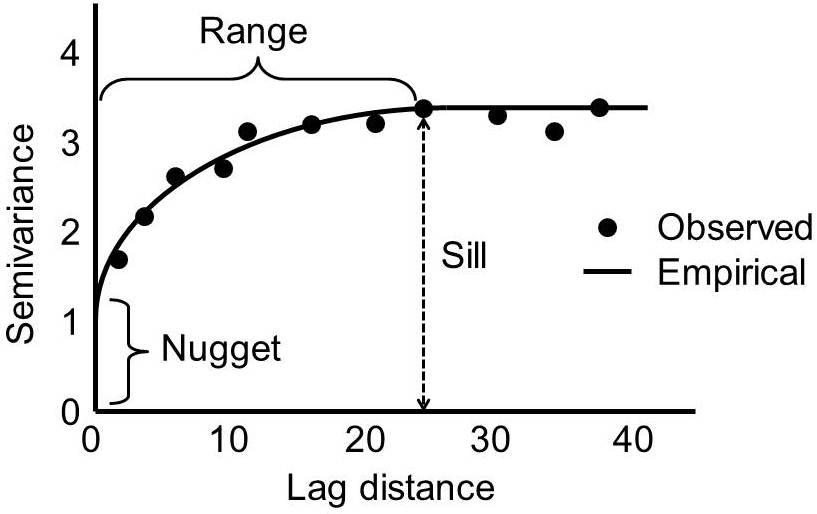
\includegraphics[width=.8\textwidth]{IMG/sp_svgm.jpg}
\end{figure}
\end{frame}
%---------------------------------------------------------------------
\begin{frame}{Empirical semivariogram}
Three main features of an estimated empirical semivariogram: 
\begin{itemize}
\item \textit{Nugget} (nugget effect) describes the micro-scale variations or measurement errors in data. Theoretically, at zero distance, $\gamma(0)=0$. However, two factors play a role here: First, $\gamma(d_1)$ is estimated over the $N(d_1)$ set of pairs, i.e. for the first interval where $ d_{ij} \in (0, d_1 ]$. Second, fitting the empirical semivariogram curve to observed values often causes the non-zero nugget.
\smallskip
\item \textit{Sill} amounts to $\lim_{d \to \infty} \gamma(d)$. The sill corresponds to variance of the stochastic field at distances where spatial dependency (which reduces $\gamma(d)$) no longer applies. $\lim_{d \to \infty} \gamma(d) = C(\bm{0}) = \textit{var}[Z(\bm{s})]$.
\smallskip
\item \textit{Range} is the spatial distance (if any) beyond which the data are not autocorrelated. In a way, range describes the strength of spatial structure -- based on where the semivariogram ``reaches'' its asymptote (sill).
\end{itemize}
\end{frame}
%---------------------------------------------------------------------
\begin{frame}{Empirical semivariogram (fitting)}
\vspace{-0.25cm}
\begin{figure}
	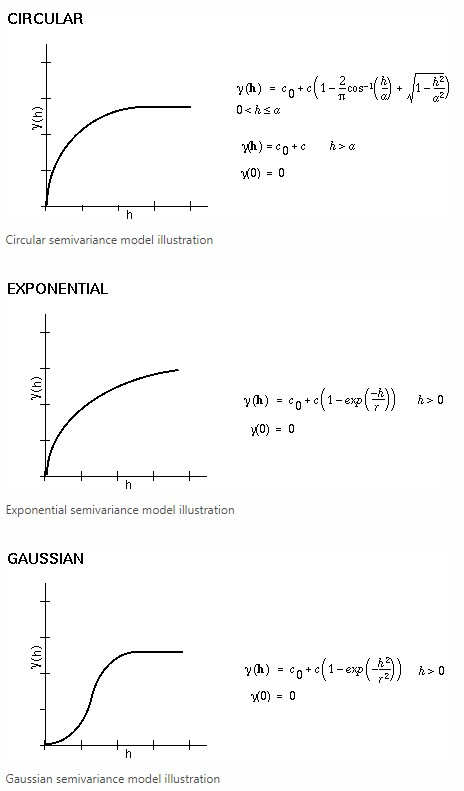
\includegraphics[width=.4\textwidth]{IMG/sp_svgm2.jpg}
\end{figure}
\end{frame}
%---------------------------------------------------------------------
\begin{frame}{Empirical semivariogram (directional semivariogram)}
\begin{figure}
	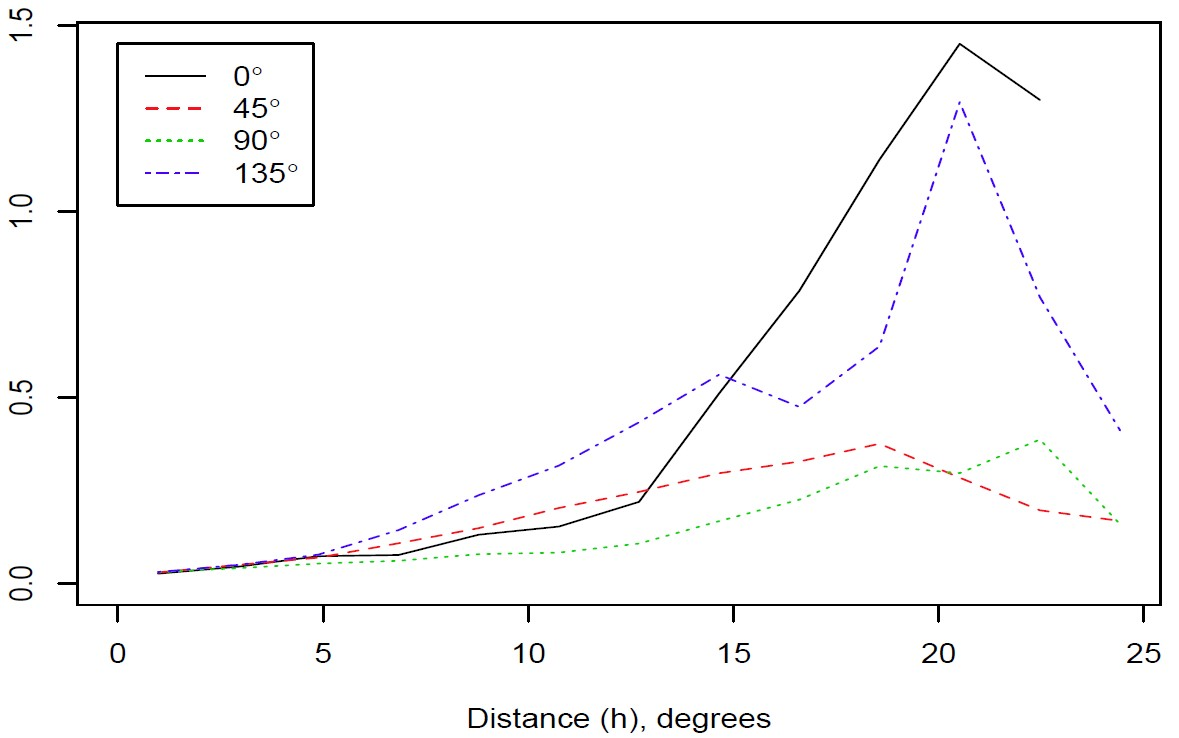
\includegraphics[width=.8\textwidth]{IMG/sp_svgm3.jpg}
\end{figure}
\end{frame}
%---------------------------------------------------------------------
\begin{frame}{Spatio-temporal stochastic processes}
The above discussion can be generalized to accommodate processes that are observed repeatedly over time. \\ \medskip 
Such observations usually exhibit both spatial and temporal dependency and variability.\\ \medskip  
Given the frequency and density limitations of empirical measurements in continuous space and time, we model our observations as realizations of a spatio-temporal random function (random field)
\begin{equation*} 
Z(\bm{s},t), \hspace{1cm} \textnormal{where~} (\bm{s},t) \in \, \mathbb{R}^d \! \times \mathbb{R} \,,
\end{equation*}
the spatio-temporal domain is indexed in space by $\bm{s} \in \mathbb{R}^d$ and in time by $t \in \mathbb{R}$. \\ \medskip 
The separation between spatial and time dimensions is substantial, which is reflected in the notation.
\end{frame}
%---------------------------------------------------------------------
\begin{frame}{Spatio-temporal stochastic processes}
Weak and intrinsic stationarity concepts can be easily expanded from spatial to spatio-temporal data. \\ \medskip
For an intrinsically stationary process $Z(\bm{s},t)$, spatio-temporal semivariograms (STSV) is:
\begin{equation*} 
\gamma(\bm{h};t) = \frac{1}{2} \textnormal{var} \left[ Z(\bm{s}_0+\bm{h} \, ; \> t_0 + t) - Z(\bm{s}_0;t_0) \right],
\hspace{1cm} (\bm{h},t) \in \, \mathbb{R}^d \! \times \mathbb{R}.
\end{equation*}
STSV does not depend on the selection of origin $(\bm{s}_0, t_0) \in \mathbb{R}^d \! \times \mathbb{R}$ (under intrinsic stationarity). \\ \medskip Also, for intrinsically stationary random fields $Z(\bm{s},t)$, the STSV $\gamma(\bm{h};t)$ is non-negative and $\gamma(\bm{0};0) = 0$.
\end{frame}
%---------------------------------------------------------------------
\begin{frame}{Empirical STSV (EU's Unemp., NUTS0, 2002---2016)}
\begin{figure}
	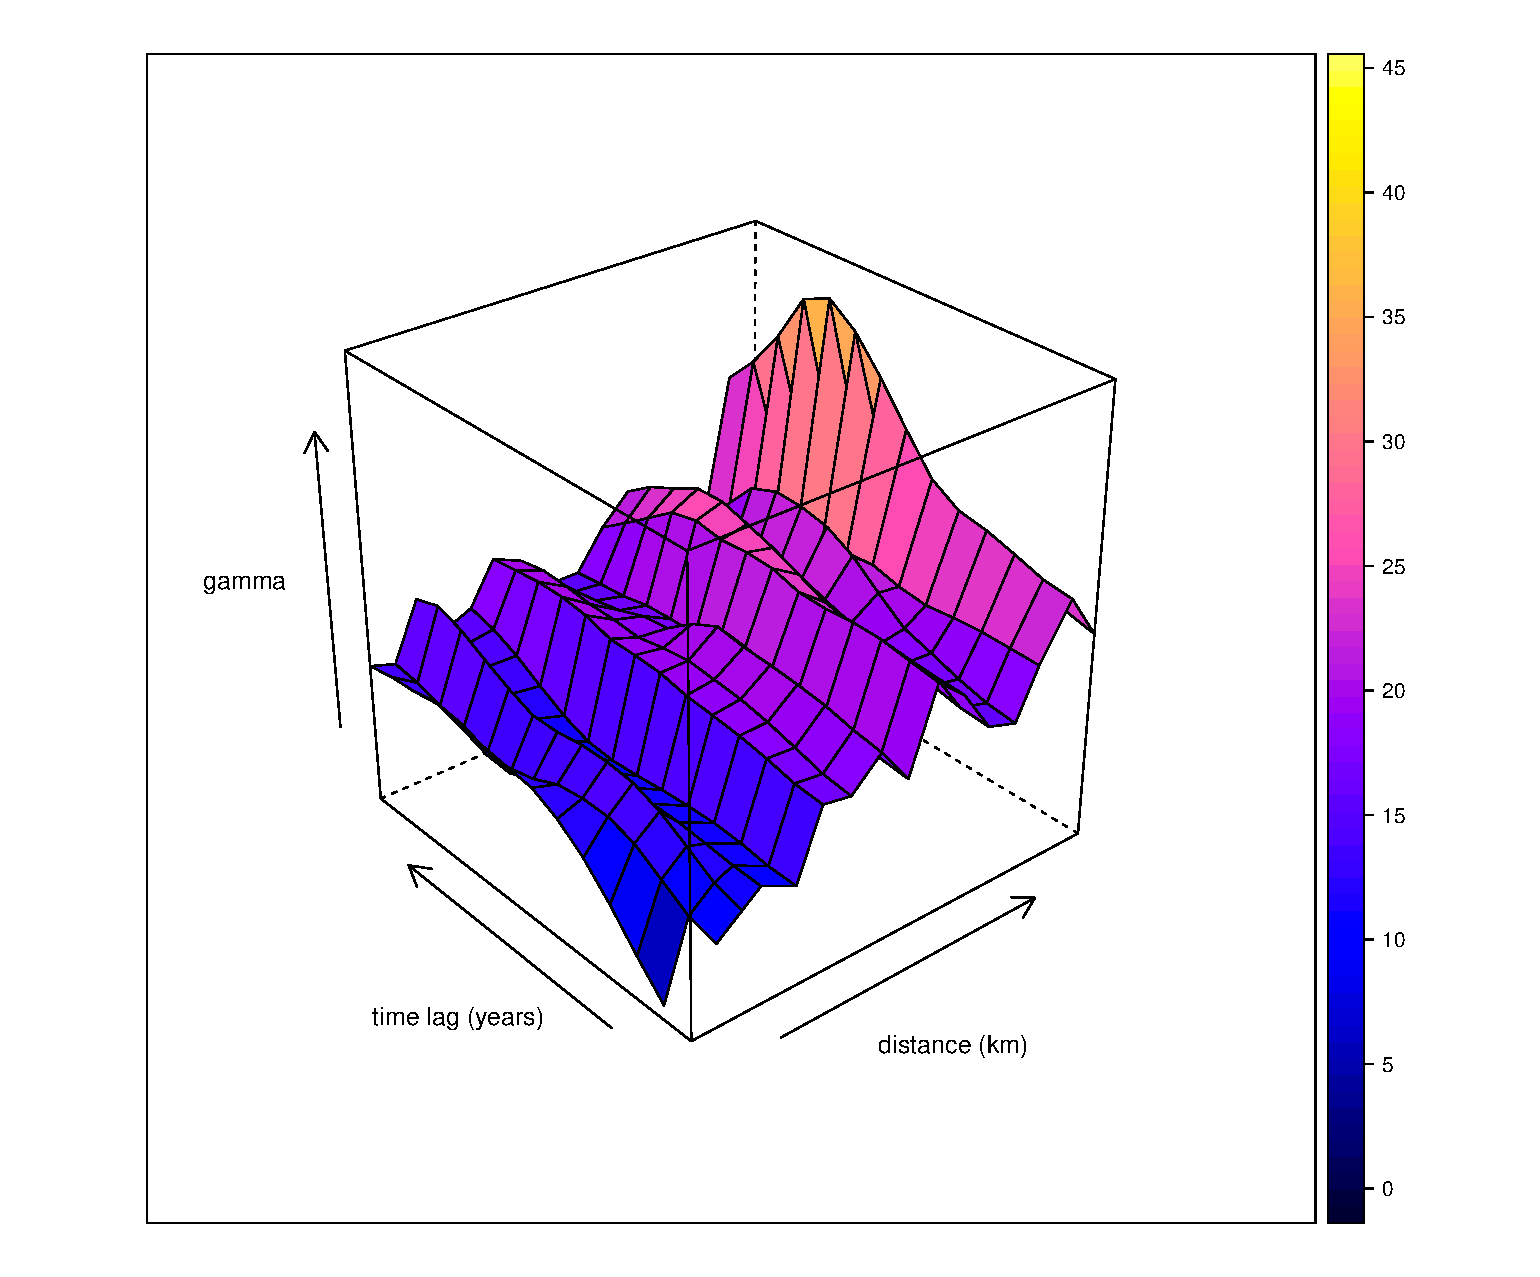
\includegraphics[width=.7\textwidth]{IMG/sp_STV.eps}
\end{figure}
\end{frame}
%---------------------------------------------------------------------























%---------------------------------------------------------------------
\begin{frame}{Prostorová autokorelace}
\begin{itemize}
\item Prostorové modely umožňují rozlišit vliv geografických faktorů (prostorová autokorelace, spill-over efekty) od působení dalších relevantních proměnných, které mohou být např. ovlivněny nástroji makroekonomické politiky.
\item Pozorování (prostorové jednotky) jsou charakterizovány geografickou polohou (geo-coded), sledujeme vzdálenosti mezi jednotkami.
\end{itemize}
\end{frame}
%---------------------------------------------------------------------
\begin{frame}{Prostorová autokorelace}
\textbf{Prostorová závislost/autokorelace – příklady}
\begin{itemize}
	\item Ceny nemovitostí závisejí na užitných vlastnostech (byt: m$^2$, počet místností, výtah, $\dots$) ale i na lokalitě. Ceny v dané lokalitě vykazují určitou míru podobnosti$\dots$ Obvykle zde platí kladná prostorová autokorelace. 
	\item Tržby benzínových pump na dálnicích závisejí na vzdálenosti od aglomerace (resp. na hustotě provozu, která se vzdáleností od aglomerace slábne). Speciální případ jednorozměrné prostorové závislosti (obvykle uvažujeme 2D vzdálenosti a závislosti).
	\item Zvýšená policejní přítomnost/aktivita v určité oblasti (okrese) sníží míru kriminality, ale může způsobit přesun nelegálních aktivit do okolních oblastí (negativní autokorelace).
	\item Makroekonomické šoky (pozitivní i negativní) se mohou "přelévat" mezi ekonomikami. 
\end{itemize}
\end{frame}
%---------------------------------------------------------------------
\begin{frame}{Prostorová autokorelace}
\begin{itemize}
	\item \textit{"Prostorová závislost popisuje vztah pozorovaného atributu (hodnota sledované proměnné) v určité oblasti vůči pozorovaným atributům v okolních oblastech."} (Fotheringham et al, 2002).
	
	\item \textit{"Prostorová autokorelace ($\dots$) je korelace mezi pozorovanými hodnotami jedné proměnné, již lze přisoudit výhradně geografické blízkosti jednotlivých pozorování ($\dots$)."} (Griffith, 2003).
\end{itemize}
\end{frame}
%---------------------------------------------------------------------
\begin{frame}{Prostorová autokorelace}
\textbf{Prostorová závislost – diskuse}
\begin{itemize}
	\item Velká část prostorových efektů (prostorové závislosti) úzce souvisí s vynechanými faktory (důležité vysvětlující proměnné modelu).
	
	\item Prostorová autokorelace - proxy proměnná pro řadu nepozorovatelných nebo obtížně kvantifikovatelných faktorů. Například, jde-li o trh práce (nezaměstnanost) v EU: 
	\begin{itemize}
		\item Dojíždění za prací mezi okresy/kraji/státy, resp. konzistentní měření tohoto jevu.
		\item Jazykové, kvalifikační, administrativní bariéry na pracovním trhu.
		\item Vzdušné vzdálenosti vs. toplogie vs. kvalita a hustota dopravní sítě. 
	\end{itemize}
	\item Prostorové modely mohou poskytnout dobře interpretovatelný a prakticky využitelný způsob analýzy makroekonomické (regionální) dynamiky.
\end{itemize}
\end{frame}
%---------------------------------------------------------------------
\section{Definice sousedících oblastí (Neighbours)}
\begin{frame}{Definice sousedících oblastí (Neighbours)}
\begin{itemize}
\item \textbf{Společná hranice (Contiguity approach)} dvě jednotky jsou definovány jako sousedící, pokud sdílejí společnou hranici (alespoň jeden bod). 	
\item \textbf{Společná hranice - zobecněná definice (Contiguity - generalized approach)}  Zobecnění je založeno na předpokladu, že oblasti, které přímo sdílejí hranici, jsou sousední oblasti prvního řádu. Za sousední oblast lze potom považovat i tzv. "sousední oblast druhého řádu" - tedy přímo nesousedící oblast, která sdílí hranici se sousedem prvního řádu. Nejvyšší přípustnou hodnotu řádu sousedící oblasti (míru vzdálenosti, míru prostorového zpoždění) lze volit arbitrárně.	
\end{itemize}
\end{frame}
%---------------------------------------------------------------------
\begin{frame}{Definice sousedících oblastí (Neighbours)}
\begin{itemize}
	\item \textbf{Sousedství podle vzdálenosti (Distance-based approach)} Dvě jednotky považujeme za sousedící, pokud jejich vzdálenost nepřesahuje předem definovanou mez (threshold). 
	\begin{itemize}
		\item Může generovat "ostrovy" (jednotky bez sousedů), pokud maximální vzdálenost mezi sousedními jednotkami je nastavena níže než je minimální vzdálenost mezi jednotkami ve výběru. 
		\item Méně vhodný přístup pro analýzu oblastí s nestejnoměrnou geografickou hustotou (různorodé velikosti a vzdálenosti). 
	\end{itemize}
	\item \textbf{Vzdálenosti mezi jednotkami měříme pomocí centroidů} - vhodně zvolených a reprezentativních bodů (míst):  
	\begin{itemize}
		\item Geografický střed oblasti, poloha  "hlavního města", střed oblasti vážený na základě hustoty obyvatel, střed založený na dopravní síti, atd.
	\end{itemize}
\end{itemize}
\end{frame}
%---------------------------------------------------------------------
\begin{frame}{Definice sousedících oblastí (Neighbours)}
\begin{figure}
	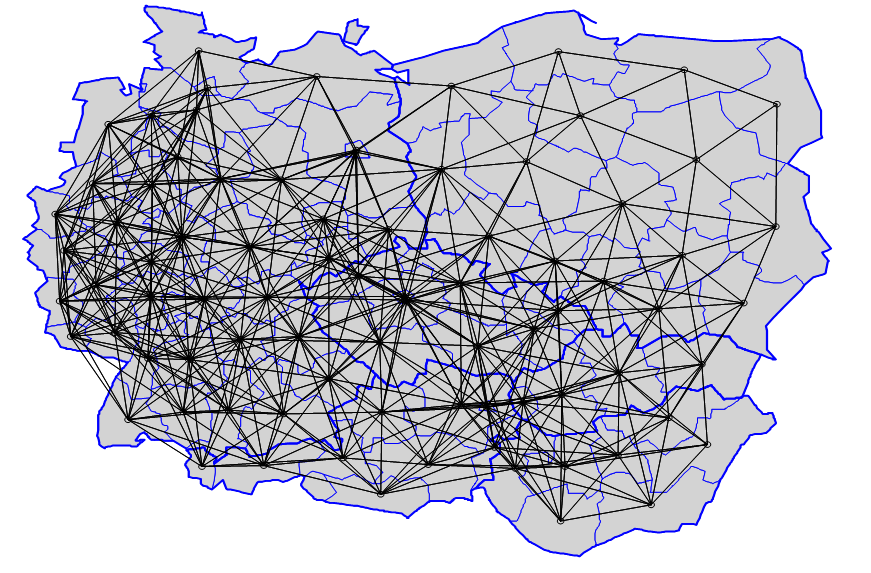
\includegraphics[width=.7\textwidth]{IMG/sp_neigb.PNG}
	\caption{Plot for distance-based neighbours (NUTS2), maximum neighbour distance threshold at 250 km}
\end{figure}
\end{frame}
%---------------------------------------------------------------------
\begin{frame}{Definice sousedících oblastí (Neighbours)}
\textbf{K-k-nejbližších sousedů(KNN)} \\
Za sousedící oblasti označíme předem stanovený počet k okolních oblastí, které jsou geograficky nejblíže. 
\begin{itemize}
	\item Řeší problémy s nestejnoměrnou geografickou hustotou (k sousedů zaručeno pro každou jednotku).
	\item Metoda obvykle vede k \textbf{asymetrickým prostorovým maticím} – obtížná interpretace sousednosti. $\dots$  existují jednoduché transformační algoritmy. 
	
	\item Příklad pro $k = 3$   (sousední oblasti vyobrazeny jen pro dvě jednotky):
	\begin{figure}
		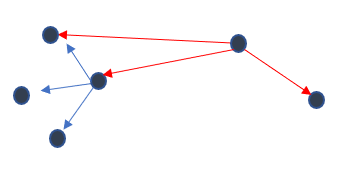
\includegraphics[width=.2\textwidth]{IMG/sp_neigb2.PNG}
	\end{figure}
\end{itemize}
\end{frame}
%---------------------------------------------------------------------
\section{Prostorové matice}
\begin{frame}{Prostorová matice – spatial matrix ($\bm{S}$)}
$$
\bm{S} = \begin{bmatrix}
0 & 1 & 1 & 1 \\
1 & 0 & 1 & 0 \\
1 & 1 & 0 & 1 \\
1 & 0 & 1 & 0
\end{bmatrix}\quad \text{příklad prostorové matice, počet jednotek: 4}$$
$$s_{ij}=
	\begin{cases}
	1, & \text{pokud jsou jednotky $i$ a $j$ sousedé.}\\
	1, & \text{nejde o sousedící jednotky}
	\end{cases}$$
\begin{itemize}
	\item Nuly na diagonále – jednotka není sama sobě sousedem.
	\item Interpetace prostorové matice: 
	\begin{itemize}
		\item 1. řádek (jednotka 1 sousedí s jednotkami 2,3,4
		\item 2. řádek jedntoka 2 sousedí s jednotkami 1,3 - ale nesousedí s jednotkou 4
		\item $\dots$ matice $\bm{S}$ je symetrická
	\end{itemize}
\end{itemize}
\end{frame}
%---------------------------------------------------------------------
\begin{frame}{Matice vah – weight matrix ($\bm{W}$)}
\vspace{-0.5cm}
$$
\bm{S} = \begin{bmatrix}
0 & 1 & 1 & 1 \\
1 & 0 & 1 & 0 \\
1 & 1 & 0 & 1 \\
1 & 0 & 1 & 0
\end{bmatrix}\rightarrow 
\bm{W}=
\begin{bmatrix}
0 & \tfrac{1}{3} & \tfrac{1}{3} & \tfrac{1}{3} \\[2pt]
\tfrac{1}{2} & 0 & \tfrac{1}{2} & 0 \\[2pt]
\tfrac{1}{3} & \tfrac{1}{3} & 0 & \tfrac{1}{3} \\[2pt]
\tfrac{1}{2} & 0 & \tfrac{1}{2} & 0
\end{bmatrix}
$$
\begin{itemize}
	\item Obvykle provedeme jednoduchou standardizaci $\bm{W}$ po řádcích: 
	$$ w_{ij} = \frac{s_{ij}}{\sum^n_{j=1} s_{ij}}$$
	$n$ - počet prostorových jednotek
	\item Nevhodné pro oblasti s heterogenní hustotou (velký vliv u oblastí s málo sousedy). 
	\item Binární indikátory $s_{ij}$ lze před standardizací zobecnit - například, místo binárních indikátorů využijeme předpoklad, že síla prostorové závislosti klesá se vzdáleností mezi jednotkami (lineárně, kvadraticky, atd.). Validita použitého prioru následně ovlivní přesnost/platnost informací, získaných prostorovou regresí.
\end{itemize}
\end{frame}
%---------------------------------------------------------------------
\begin{frame}{Matice vah – weight matrix ($\bm{W}$)}
$$
\bm{W}=
\begin{bmatrix}
0 & \tfrac{1}{3} & \tfrac{1}{3} & \tfrac{1}{3} \\[2pt]
\tfrac{1}{2} & 0 & \tfrac{1}{2} & 0 \\[2pt]
\tfrac{1}{3} & \tfrac{1}{3} & 0 & \tfrac{1}{3} \\[2pt]
\tfrac{1}{2} & 0 & \tfrac{1}{2} & 0
\end{bmatrix}
$$
\begin{itemize}
	\item Každý řádek matice $\bm{W}$ "tvoří" očekávanou hodnotu sledované proměnné - např. $y_i$ - na základě váženého průměru hodnot sousedních jednotek. Například:
	\begin{align*}
	\hat{y}_1 & =  \tfrac{1}{3} y_2 + \tfrac{1}{3} y_3 + \tfrac{1}{3} y_4 \\
	\dots \\
	\hat{y}_4 & = \tfrac{1}{2} y_1  + \tfrac{1}{3} y_3 
	\end{align*}
	\item Pozorované hodnoty proměnných u prostorových jednotek lze využít pro predikci příslušných hodnot u sousedících jednotek.
\end{itemize}
\end{frame}
%---------------------------------------------------------------------
\section{Moran's I, Geary's C}
\begin{frame}{Moran's $I$}
Nejčastěji uváděný a používaný test prostorové nezávislosti
$$I(x)_t = \big( \frac{n}{s}\big) \bm{x}^T_t \bm{W} \bm{x}_t (\bm{x}_t^T\bm{x}_t)^{-1}$$
kde $\bm{x}_t$ je vektor $n$ prostorových pozorování (jednotek) proměnné $x$ v čase $t$. 
$$S = \sum_{i=1}^n\sum_{j=1}^n w_{ij}$$
$S$ je standardizační faktor – součet všech členů matice $\bm{W}$. \\
$H_0 :$ absence prostorové závislosti, prostorová náhodnost (spatial randomness) \\
Očekávaná hodnota statistiky  $I(x)_t$ při platnosti $H_0 : \frac{-1}{(n-1)} $.\\
Pomocí $Var(I(x)_t)$ vypočteme $z$-poměr a testujeme statistickou významnost: zda jsou si sousedící jednotky více podobné, než by odpovídalo platné $H_0$. \\
Znaménko Moran's $I$ statistiky rozlišuje mezi pozitivní a negativní prostorovou autokorelací.
\end{frame}
%---------------------------------------------------------------------
\begin{frame}{Geary's $C$}
Geary's C je definován jako:
$$C = \frac{(N-1)\sum_i \sum_j w_{ij} (X_i - X_j)^2}{2W\sum_i (X_i -\bar{X})^2}$$
kde $N$ je počet prostorových jednotek; $X$ zkoumaná proměnná, $\bar{X}$ je průměrná hodnota, $w_{ij}$ jsou prvky matice vah a $W$ je součet všech prvků $w_{ij}$ . 
\begin{itemize}
	\item Geary's $C$ nabývá hodnotu mezi 0 a 2. 1 představuje prostorovou nezávislost. Hodnoty nižší než 1 znamenají pozitivní prostorovou autokorelaci, narůstající směrem k nule. Hodnoty vyšší než 1, indikují negativní prostorovou autokorelaci.
	\item Geary's $C$ je inverzně spjat se statistikou Moran's $I$. Zatímco Moran's $I$ popisuje celkovou prostorovou autokorelaci, Geary's $C$ je více citlivý na lokální vlivy.
\end{itemize}
\end{frame}
%---------------------------------------------------------------------
\section{Základní modely prostorové regrese}
\begin{frame}{Základní modely prostorové regrese}
\begin{figure}
	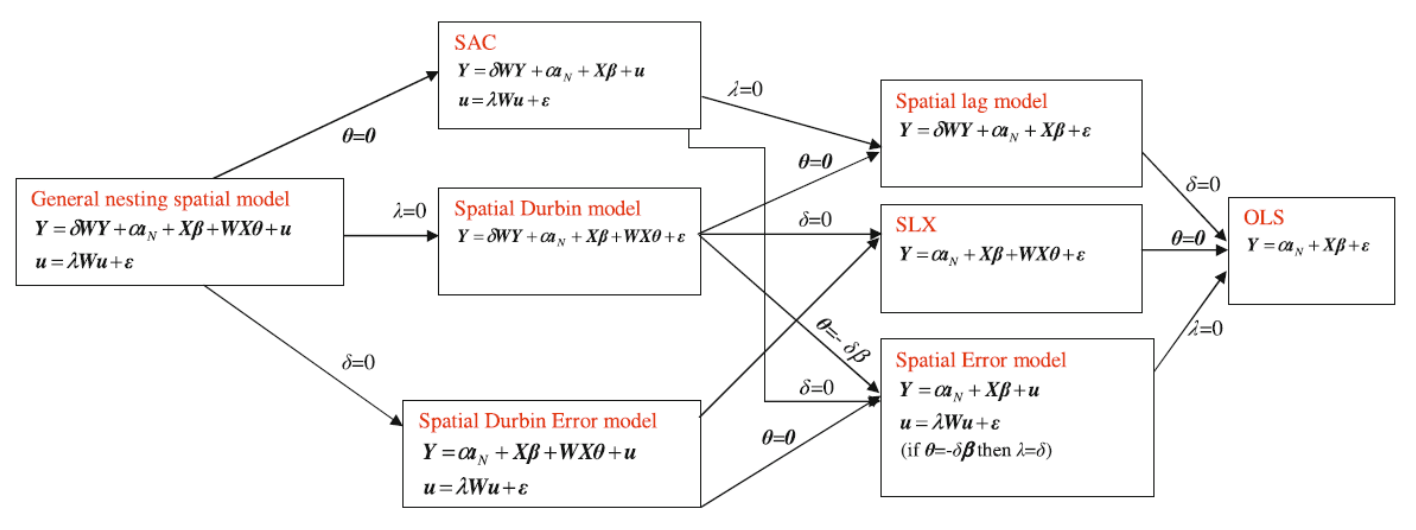
\includegraphics[width=.9\textwidth]{IMG/sp_reg.PNG}
	\caption{The rleationship betwee different spatial dependence models for cross-section data (source Halleck Vega and Elhorst 2012)}
\end{figure}
\end{frame}
%---------------------------------------------------------------------
\begin{frame}{Základní modely prostorové regrese}
\begin{itemize}
	\item \textbf{Prostorová autokorelace závislé proměnné}
	$$\bm{y}_t = \rho \bm{W}\bm{y}_t + \dots$$
	$\bm{Wy}_t$ popisuje prostorovou interakci mezi endogenními proměnnými modelu
	$\textit{SpatialLag}(y_{it}) = \bm{w}^T_i \bm{y}_t$, kde je $ \bm{w}^T_i$ řádek matice $\bm{W}$, $\bm{y}_t$ jsou pozorování $y$ v čase $t$.\\
	$\rho$ je koeficient prostorové autokorelace závislé proměnné (skalár); obvykle $\rho \in (-1,1)$.
	\item \textbf{Prostorová autokorelace regresorů}
	$$\bm{y}_t = \dots + \bm{X}_t \bm{\beta} + \bm{W}\bm{X}_t \bm{\theta} + \dots$$
	$\bm{X}$ je obvyklá matice regresorů, $\bm{WX}$ popisuje exogenní prostorové interakce mezi nezávislými proměnnými, $\bm{\beta}$ a $\bm{\theta}$ jsou vektory ($k\times 1$) neznámých parametrů, které se snažíme odhadnout.
\end{itemize}
\end{frame}
%---------------------------------------------------------------------
\begin{frame}{Základní modely prostorové regrese}
\begin{itemize}
	\item \textbf{Prostorová autokorelace náhodné složky} 
	$$\bm{u}_t = \lambda \bm{Wu}_t + \bm{\epsilon}_t$$
	 $\bm{Wu}_t$ popisuje prostorovou interakci mezi náhodnými složkami prostorových jednotek \\
	 $\lambda$ je koeficient prostorové autokorelace náhodné složky, resp. vynechaných prostorově  závislých vysvětlujících proměnných (skalár) \\
	 $\bm{\epsilon}_t$ vektor skutečných náhodných složek – prostorově nezávislá část náhodných složek.
	\item \textbf{Volba modelu se zahrnutím prostorové autokorelace} \\
		Konkrétní typ modelu volíme pomocí omezujících předpokladů: položíme $\rho,\theta$ nebo $\lambda$ rovné nule.
	Omezující předpoklady lze testovat. 
\end{itemize}
\end{frame}
%---------------------------------------------------------------------
\begin{frame}{Základní modely prostorové regrese}
\textbf{Spatial lag model}
\begin{itemize}
	\item Zajímá-li nás prostorová interakce mezi pozorovanými hodnotami závislé proměnné. Prostorovou závislost (strukturu) zde předpokládáme pouze u endogenní proměnné modelu. Model, resp. jeho redukovaná forma, mají tvar: 
	\begin{align*}
	\bm{y}_t & = \rho \bm{Wy}_t + \bm{X}_t\bm{\beta}+ \bm{u}_t\\
	(\bm{I} - \rho \bm{W}) \bm{y}_t & = \bm{X}_t \bm{\beta} + \bm{u}_t
	\end{align*}
	\item Koeficienty $\rho$ i $\bm{\beta}$ jsou odhadnuty metodou maximální věrohodnosti (MLE). Koeficienty  $\bm{\beta}$  pomáhají vysvětlit tu část variability $\bm{y}$, která není vysvětlena prostorově.	
\end{itemize}
\end{frame}
%---------------------------------------------------------------------
\begin{frame}{Základní modely prostorové regrese}
\textbf{Spatial Durbin model}
\begin{itemize}
	\item Vznikne rozšířením specifikace Spatial lag model o prostorové interakce mezi regresory: 
		\begin{align*}
		\bm{y}_t & = \rho \bm{Wy}_t + \bm{X}_t\bm{\beta}+ \bm{Wy}_t\bm{X}_t\bm{\theta} +  \bm{u}_t\\
		(\bm{I} - \rho \bm{W}) \bm{y}_t & = \bm{X}_t \bm{\beta} + \bm{Wy}_t\bm{X}_t\bm{\theta}+ \bm{u}_t
		\end{align*}
\end{itemize}
\end{frame}
%---------------------------------------------------------------------
\begin{frame}{Základní modely prostorové regrese}
\textbf{Spatial error model}
	\begin{align*}
	\bm{y}_t & =   \bm{X}_t\bm{\beta}+  \bm{u}_t, \qquad \bm{u}_t = \lambda  \bm{Wu}_t + \bm{\epsilon}_t\\
	\bm{y}_t & = \bm{X}_t\bm{\beta}+ \lambda\bm{Wy}_t\bm{u}_t+  \bm{\epsilon}_t\\
	(\bm{I} - \lambda \bm{W}) \bm{y}_t & = (\bm{I} - \lambda \bm{W}) \bm{X}_t \bm{\beta} + \bm{\epsilon}_t
	\end{align*}
\begin{itemize}

	\item I v případě, kdy se nezajímáme o prostorové interakce mezi pozorovanými proměnnými, můžeme zlepšit vlastnosti odhadu pomocí prostorově závislých chyb.
	\item Interakce v rámci náhodné složky nevyžadují teoretické zdůvodnění interakčního procesu, předpokládáme existenci prostorově závislých proměnných, nezahrnutých do modelu
\end{itemize}
\end{frame}
%---------------------------------------------------------------------
\begin{frame}{Prostorové modely:  stacionarita/stabilita}
\textbf{Stacionarita}
\begin{itemize}
\item Neformálně: pro každou oblast je počet sousedících oblastí omezený (malý)
\item Řádkové (a sloupcové) součty matice $\bm{S}$ jsou konečné a omezené, i když počet uvažovaných prostorových jednotek $n$ roste neomezeně.
\item Korelace mezi dvěma prostorovými jednotkami konverguje k nule s rostoucí vzdáleností mezi těmito jednotkami.
\item Formální podmínky stacionarity (pro $\rho, \lambda$ a $\bm{W}$ ) viz \href{https://www.google.cz/url?sa=t&rct=j&q=&esrc=s&source=web&cd=1&cad=rja&uact=8&ved=0ahUKEwjjwvLCk8bLAhXEvXIKHWSHBxsQFgggMAA&url=http://www.springer.com/cda/content/document/cda_downloaddocument/9783642403392-c2.pdf?SGWID\%3D0-0-45-1432965-p175381976&usg=AFQjCNGpme8ofJQzd46BCJVsUEio6oKIzQ&sig2=LlarV9wYhELGcTPiqzfRgg}{Elhorst (2014)}.
\end{itemize}
\end{frame}
%---------------------------------------------------------------------
\begin{frame}{Prostorové modely:  stacionarita/stabilita}
\textbf{Stabilita odhadů}
\begin{itemize}
	\item Matice $\bm{S}$, resp. matice $\bm{W}$ není odhadována, musíme ji stanovit předem. Odhadnuté koeficienty $\bm{\beta}$, resp. $\bm{\theta}$ závisejí na zvolené matici $\bm{W}$.
	\item "Řešení": regresní modely odhadujeme opakovaně, pokaždé s trochu jinak definovanou maticí $\bm{W}$ a porovnáváme vlastnosti jednotlivých odhadů.
    \item Tento postup zaručuje pouze lokální optimum (určíme nejlepší z porovnávaných modelů podle zvoleného kritéria), nikoliv globální optimum.
	\end{itemize}
\end{frame}
%---------------------------------------------------------------------
\section{Přímé a nepřímé efekty (Spill-overs)}
\begin{frame}{Přímé a nepřímé efekty (Spill-overs)}
\begin{itemize}
	\item $(\bm{I} - \rho \bm{W}) \bm{y}_t = \bm{X}_t \bm{\beta} + \bm{W}\bm{X}_t\bm{\theta} + \alpha \bm{\iota} +\bm{u}_t$ \quad $ \alpha \bm{\iota}$ je vektor úroňových konstant
	\item $\bm{y}_t = (\bm{I} - \rho \bm{W})^{-1} (\bm{X}_t\bm{\beta} + \bm{W}\bm{X}_t \bm{\theta})+ \bm{R}_t$ \quad 
	$\bm{R}_t$ obsahuje náhodnou složku i intercept 
\end{itemize}
Derivaci $E(\bm{y}_t)$ podle $k$-té vysvětlující proměnné $\bm{x}_{kt}$ lze zapsat jako:\\(časový index $t$ pro jednuduchost vynecháme)

\begin{align*} \bigg[\frac{\partial E(\bm{y})}{\partial \bm{x}_{1,k}} \dots \frac{\partial E(\bm{y})}{\partial \bm{x}_{N,k}}\bigg] & =
\begin{bmatrix}
\frac{\partial E(y_1)}{\partial \bm{x}_{1,k}} & \dots & \frac{\partial E(y_1)}{\partial \bm{x}_{N,k}} \\
\vdots & \ddots & \vdots \\
\frac{\partial E(y_N)}{\partial \bm{x}_{1,k}} & \dots & \frac{\partial E(y_N)}{\partial \bm{x}_{N,k}}
\end{bmatrix} = \\
& = (\bm{I} - \rho \bm{W})^{-1} 
\begin{bmatrix}
\beta_k & w_{12}\theta_k & \dots & w_{1N}\theta_k \\
w_{21}\theta_K & \beta_k & \dots & w_{2N}\theta_k \\
\vdots & \ddots & \ddots & \vdots \\
w_{N1}\theta_k & w_{N2}\theta_k & \dots & \beta_k 
\end{bmatrix}
\end{align*}
\end{frame}
%---------------------------------------------------------------------
\begin{frame}{Přímé a nepřímé efekty (Spill-overs)}
$$ \bigg[\frac{\partial E(\bm{y})}{\partial \bm{x}_{1,k}} \dots \frac{\partial E(\bm{y})}{\partial \bm{x}_{N,k}}\bigg] =
 (\bm{I} - \rho \bm{W})^{-1} 
\begin{bmatrix}
\beta_k & w_{12}\theta_k & \dots & w_{1N}\theta_k \\
w_{21}\theta_K & \beta_k & \dots & w_{2N}\theta_k \\
\vdots & \ddots & \ddots & \vdots \\
w_{N1}\theta_k & w_{N2}\theta_k & \dots & \beta_k 
\end{bmatrix}
$$
%---------------------------------------------------------------------
\begin{itemize}
	\item Změním-li hodnotu vysvětlující proměnné $x_k$ u $i$-té prostorové jednotky (změna $x_{ik}$), dojde ke změně očekávané hodnoty $y_i$ - \textbf{přímý efekt} a zároveň dojde ke změně očekávané hodnoty $y$ u dalších prostorových jednotek – \textbf{nepřímý efekt}. 
	\item Diagonální prvky matice (RHS) představují přímé efekty, prvky mimo diagonálu jsou nepřímé efekty
\end{itemize}

\end{frame}
%---------------------------------------------------------------------
\begin{frame}{Přímé a nepřímé efekty (Spill-overs)}
$$ \bigg[\frac{\partial E(\bm{y})}{\partial \bm{x}_{1,k}} \dots \frac{\partial E(\bm{y})}{\partial \bm{x}_{N,k}}\bigg] =
(\bm{I} - \rho \bm{W})^{-1} 
\begin{bmatrix}
\beta_k & w_{12}\theta_k & \dots & w_{1N}\theta_k \\
w_{21}\theta_K & \beta_k & \dots & w_{2N}\theta_k \\
\vdots & \ddots & \ddots & \vdots \\
w_{N1}\theta_k & w_{N2}\theta_k & \dots & \beta_k 
\end{bmatrix}
$$

\begin{itemize}
	\item Přímé a nepřímé efekty se liší pro jednotlivé prostorové jednotky ($i$).
	\begin{itemize}
	\item 	Přímé efekty se liší, protože diagonální prvky $(\bm{I} - \rho \bm{W})^{-1} $ jsou různé, pokud $\rho \neq 0$.
	\item Nepřímé efekty se liší, protože prvky mimo diagonálu matice $\bm{W}$, resp. $(\bm{I} - \rho \bm{W})^{-1}$ jsou různé, pokud $\rho \neq 0$ a/nebo $\theta_k \neq 0$
\end{itemize}
	$$ (\bm{I} - \rho \bm{W})^{-1} = \bm{I} + \rho\bm{W} + \rho^2\bm{W}^2 + \rho^3\bm{W}^3 + \dots$$

	\item Diagonální prvky matice (RHS) představují přímé efekty, prvky mimo diagonálu jsou nepřímé efekty
\end{itemize}
\end{frame}
%---------------------------------------------------------------------
\begin{frame}{Přímé a nepřímé efekty (Spill-overs)}
$$ \bigg[\frac{\partial E(\bm{y})}{\partial \bm{x}_{1,k}} \dots \frac{\partial E(\bm{y})}{\partial \bm{x}_{N,k}}\bigg] =
(\bm{I} - \rho \bm{W})^{-1} 
\begin{bmatrix}
\beta_k & w_{12}\theta_k & \dots & w_{1N}\theta_k \\
w_{21}\theta_K & \beta_k & \dots & w_{2N}\theta_k \\
\vdots & \ddots & \ddots & \vdots \\
w_{N1}\theta_k & w_{N2}\theta_k & \dots & \beta_k 
\end{bmatrix}
$$
%---------------------------------------------------------------------
\begin{itemize}
\item \textbf{Interpretace odhadnutého prostorového regresního modelu – vždy na základě přímých a nepřímých efektů}. 
\item Koeficient $\beta_k$ nepopisuje chování závislé proměnné $y_i$ při změně $x_{ik}$ "správně".
\item Statistickou významnost přímých efektů můžeme testovat viz \href{https://www.google.cz/url?sa=t&rct=j&q=&esrc=s&source=web&cd=1&cad=rja&uact=8&ved=0ahUKEwjjwvLCk8bLAhXEvXIKHWSHBxsQFgggMAA&url=http://www.springer.com/cda/content/document/cda_downloaddocument/9783642403392-c2.pdf?SGWID\%3D0-0-45-1432965-p175381976&usg=AFQjCNGpme8ofJQzd46BCJVsUEio6oKIzQ&sig2=LlarV9wYhELGcTPiqzfRgg}{Elhorst (2014)}.	
\end{itemize}
\end{frame}
%---------------------------------------------------------------------
\begin{frame}{Přímé a nepřímé efekty (Spill-overs)}
\begin{itemize}
	\item Ukázkový výstup odhadu přímých a nepřímých efektů (LeSage/Pace, 2009):
	$$\bm{y} = (\bm{I} - \rho \bm{W})^{-1} \bm{X}\bm{\beta} + (\bm{I} - \rho \bm{W})^{-1} \bm{\epsilon}$$
	$\dots$ jednoduchá regrese $y$ na $x$, použita prostorová regrese: \\
	Spatial lag model.
	
	\end{itemize}
\begin{table}[]
\centering
\caption{Spatial partitioning of direct, indirect and total   impacts}
\begin{tabular}{llll}
&         &          &             \\
                                                                                                       & Mean    & Std. dev & t-statistic \\
Direct effect                                                                                          & 0.586   & 0.0148   & 39.6106     \\
Indirect effect                                                                                        & 1.08414 & 0.0587   & 18.4745     \\
Total effect                                                                                           & 1.67    & 0.0735   & 22.7302    
\end{tabular}
\end{table}
\end{frame}
%---------------------------------------------------------------------
\begin{frame}{Přímé a nepřímé efekty (Spill-overs)}

$$ \bigg[\frac{\partial E(\bm{y})}{\partial \bm{x}_{1,k}} \dots \frac{\partial E(\bm{y})}{\partial \bm{x}_{N,k}}\bigg] =
(\bm{I} - \rho \bm{W})^{-1} 
\begin{bmatrix}
\beta_k & w_{12}\theta_k & \dots & w_{1N}\theta_k \\
w_{21}\theta_K & \beta_k & \dots & w_{2N}\theta_k \\
\vdots & \ddots & \ddots & \vdots \\
w_{N1}\theta_k & w_{N2}\theta_k & \dots & \beta_k 
\end{bmatrix}
$$
\begin{itemize}
	\item \textbf{Nevýhody, omezení modelů založených na prostorové závislosti:}
	\item Poměr přímého a nepřímého efektu nezávisí na $\beta_k$ - je dán pouze na základě matice $\bm{W}$ a hodnoty $\rho$. 
	\item Tento poměr je stejný pro všechny vysvětlující proměnné (resp. příslušné přímé a nepřímé efekty).
\end{itemize}

\end{frame}
%---------------------------------------------------------------------
\section{Identifikace hotspotů a coldspotů}
\begin{frame}{Identifikace "hotspotů" a "coldspotů"}
\begin{itemize}
	\item \textbf{Getis-Ord $G^\ast_i$}
	$$ G^\ast_i = \frac{\sum_{j=1}^n w_{i,j} x_j - \bar{X} \sum_{j=1}^n w_{i,j}}{S \quad\sqrt[]{\frac{[n\sum_{j=1}^n w^2_{i,j}-(\sum_{j=1}^n w_{i,j})^2]}{n-1}}}$$
	$$ \bar{X} = \frac{\sum_{j=1}^n x_j}{n}, \quad S = \sqrt[]{\frac{\sum_{j=1}^n x^2_j}{n}-(\bar{X})^2} $$
	\item $x_j$ je hodnota sledované proměnné v $j$-té jednotce, $w_{i,j}$ jsou prvky matice $\bm{W}$,  $n$ je počet prostorových jednotek.
	\item $G^\ast_i$ statistika se používá pouze pro kladnou prostorovou autokorelaci a umožňuje identifikovat prostorové shluky jednotek, které mají podobné hodnoty, jež jsou vysoké nebo nízké vůči průměrné pozorované hodnotě – hotspoty a coldspoty.\\(Getis – Ord 1992).
\end{itemize}
\end{frame}
%---------------------------------------------------------------------
\begin{frame}{Identifikace "hotspotů" a "coldspotů"}
\begin{figure}
	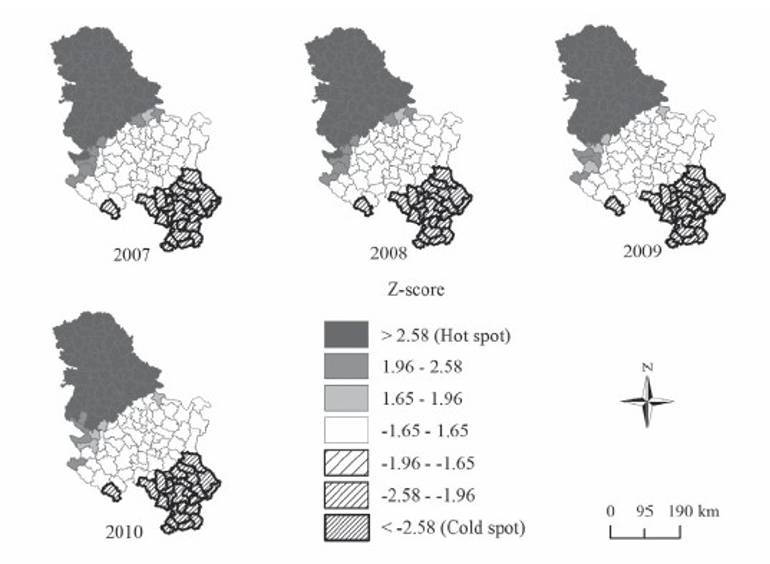
\includegraphics[width=.7\textwidth]{IMG/sp_coldspot.PNG}
	\caption{Spatial clusters (hot and cold spots) of the municipalities in Serbia by the level of average monthly net earning from 2001 to 2010 (at fix distance of 210 km)}
\end{figure}
\end{frame}
%---------------------------------------------------------------------
\begin{frame}{Identifikace "hotspotů" a "coldspotů"}
	$$ G^\ast_i = \frac{\sum_{j=1}^n w_{i,j} x_j - \bar{X} \sum_{j=1}^n w_{i,j}}{S \quad \sqrt[]{\frac{[n\sum_{j=1}^n w^2_{i,j}-(\sum_{j=1}^n w_{i,j})^2]}{n-1}}}$$
\begin{itemize}
	\item $ G^\ast_i$ je lokální statistika – spočtená pro každou prostorovou jednotku, jedná se o tzv. $z$-poměr ($z$-score).
	\item $ G^\ast_i$ popisuje statistickou významnost prostorového shlukování. Vysoká pozitivní hodnota $G^\ast_i$ indikuje koncentraci vysokých hodnot u sousedících prostorových jednotek (hotspot). Naopak, negativní hodnoty indikují výskyt tzv. coldspotu.
	\item Hodnoty blízké nule naznačují, že jednotka není součástí žádného prostorového shluku.
	
\end{itemize}
\end{frame}
%---------------------------------------------------------------------
\section{Prostorová regrese v R}
\begin{frame}{Prostorová regrese v R}
\begin{itemize}
	\item Knihovna \{spdep\} 
	\begin{itemize}
		\item Různé typy prostorových modelů
		\item Testy prostorové nezávislosti, identifikace prostorových shluků,$\dots$
	\end{itemize}
	\item	Knihovna \{splm\}
	\begin{itemize}
		\item Prostorová regrese na panelových datech
	\end{itemize}
	\item Knihovna \{ggplot2\} + další nutné knihovny
	\begin{itemize}
		\item Kartogramy (infomapy) / choropleth maps
	\end{itemize}
\end{itemize}
 \begin{figure}
 	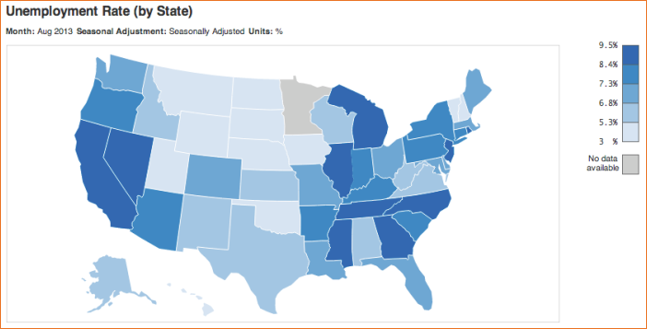
\includegraphics[width=.5\textwidth]{IMG/sp_unemp.PNG}
 \end{figure}

\end{frame}

%---------------------------------------------------------------------


\end{document}